\section{Framework overview\label{section:background-multi-agent-systems-and-behavior-modeling}}

Modeling software systems calls for rich models that cover the structural, intentional and behavioral dimensions of the system~\cite{VanLamsweerde:2000}. Our framework integrates these co-related dimensions with an emphasis on the behavioral one. We start with a guided tour along those dimensions before discussing how multiple models actually fit together in a coherent way.

\subsection{Capturing multiple views of the system\label{subsection:background-multiple-views}}

%%% The structural view

\noindent \textbf{The structural view} -- A system is commonly seen as being made of active components, called \emph{agents}, that behave and interact so as to fulfill system goals; they need to restrict their behavior so as to ensure the goals they are responsible for~\cite{Feather:1987}. Some of them are human agents (e.g. passenger in Fig.\ref{image:train-scenario-all-agents}); others are physical or electronic devices (e.g. train doors and actuators); others are software components (the software controller).

In addition to the notion of \emph{system}, that encompasses all agents, the literature makes use of specific terms to distinguish between certain agents and/or agent aggregations. In~\cite{VanLamsweerde:2009} for example, the \emph{software-to-be} denotes software agent(s) that need to be developed (the automated controller, for example) while the other agents compose its \emph{environment}. Another boundary consists in distinguishing the software together with its input and output devices from the other agents. This boundary, depicted with a dashed line in Fig.~\ref{image:train-scenario-all-agents}, corresponds to the distinction between the \emph{world} and the \emph{machine}~\cite{Jackson:1995}.

The thesis sticks to very basic notions of structural modeling. The interfaces among the agents composing the system consist of messages, called \emph{events}, that the agents can send or receive (see the behavioral dimension below). For sake of simplicity we assume that event labels uniquely determine agent interactions. We do not consider specific abstractions for modeling agent interfaces and boundaries, like context diagrams~\cite{Jackson:1995} and events structured in terms of attributes.

As illustrated by the \emph{Machine} boundary in Fig.~\ref{image:train-scenario-all-agents}, a set of agents can be aggregated into a new one of coarser granularity. Events can then be partitioned among internal, boundary and external events. The boundary events form the new agent's interface. The surrounding box can be seen as a white or a black-box dependent on whether internal events are shown or hidden, respectively. The composition and hiding operators on state machines support such structural mechanisms on the behavioral side (see Section~\ref{section:background-state-machines}). For a more precise description of structural models that nicely fit our framework the reader can refer to~\cite{Magee:1995}.

%%% The behavioral view

\noindent \textbf{The behavioral view} -- Behaviors capture the dynamic interactions among the agents forming the system; they will be modeled as sequences of events. In an interaction, an event is \emph{synchronously} sent by a source agent and received by a target agent. The same event can in fact be received by several agents at once; a form of \emph{broadcasting} is thus supported. 

Typical examples and counterexamples of system behavior are specified through positive and negative scenarios involving agent instances, like the one in Fig.~\ref{image:train-scenario-all-agents}. The Message Sequence Charts (MSC) notation will be used to capture scenarios~\cite{ITU:1996}. Higher-level scenarios will be supported by introducing sequences and loops in such descriptions.

In addition to the partial behavior description linking agent instances, the complete behavior of each agent will be modeled at class level through a form of state machine known as labeled transition systems (LTS)~\cite{Keller:1976, Milner:1989}. The behavior of the entire system is obtained by parallel composition~\cite{Hoare:1985} of the agent LTSs. Behavior  projection on specific agents is also supported, in order to get the zoom-in/zoom-out facilities as suggested before.

This thesis will focus on \emph{determinate} agents~\cite{Engelfriet:1985}; these are agents whose observable behavior can be captured with the sole use of \emph{deterministic} transition systems (see Section~\ref{section:background-state-machines}).
\begin{itemize} 
\item This restriction results in a simple and intuitive framework, for easier accessibility to stakeholders involved in the early phases of system design. 
\item It also allows us to formalize behaviors with standard \emph{trace theory} \cite{Hoare:1985} and stick ourselves to the simplest notion of behavior equivalence, namely \emph{trace equivalence}~\cite{Engelfriet:1985}. 
\item Agent and system behaviors can then be captured by the class of \emph{prefix-closed} regular languages, a subclass of the well-studied \emph{regular} languages~\cite{Hopcroft:1979, Aho:1986}. Further to enabling the reuse of standard results from automaton theory, this paves the way to the use of grammar inference~\cite{Gold:1978} for behavior model synthesis (see chapter~\ref{chapter:inductive-synthesis}). 
\end{itemize}

%%% The intentional view

\noindent \textbf{The intentional view} -- This view is aimed at capturing \emph{why} the system is needed. A \emph{goal} is a prescriptive statement of intent whose satisfaction requires the collaboration of system agents. Unlike goals, \emph{domain properties} are descriptive statement about the environment -- such as physical laws, organizational rules, etc. Goal models are AND/OR graphs that capture how functional and non-functional goals contribute positively or negatively to each other~\cite{VanLamsweerde:2000, VanLamsweerde:2004}.

The thesis will focus on behavioral goals. A \emph{behavioral} goal implicitly defines a maximal set of admissible system behaviors. Unlike \emph{soft} goals, such goals can be established in a clear-sense (refer to~\cite{VanLamsweerde:2009} for a taxonomy of goals). For model synthesis the thesis will only consider goals and domain properties that can be formalized as \emph{safety} properties in linear temporal logic (LTL)~\cite{Manna:1992}. A safety property stipulates that some ``bad thing'' may never happen. If such a ``bad thing'' happens in an infinite sequence, then it must also do so after some finite prefix and must be irremediable~\cite{Alpern:1986, Giannakopoulou:1999}. Interestingly, the class of system behaviors satisfying safety properties can be expressed through labeled transition systems; behavioral goals and domain properties can therefore be integrated in our framework without much additional machinery.

For the modeler, goals are best captured through state-based abstractions (e.g. ``the train may be \emph{moving} only if the doors are \emph{closed}''). In contrast, the formal behavioral view is event-based (e.g. ``the controller issues a \emph{start} command after having issued a \emph{close-doors} command''). 

\emph{Fluents} will be used as an effective way for reconciling these two para-digms \cite{Miller:2002}; they capture state-based propositions in terms of the occurrence of events (see Section~\ref{section:background-fluents}). Behavioral goals will therefore be formalized in Fluent Linear Temporal Logic (FLTL)~\cite{Giannakopoulou:2003}, a flavor of linear temporal logic where atomic propositions are fluents. The structuring of goals in goal graphs and their assignment to agents will not be considered in the thesis.

%%% The operational view

\noindent \textbf{The operational view} -- This view aims at capturing processes which agents are involved in. Processes will be made of tasks and decisions. A \emph{task} is a unit of work to be performed by collaboration of the agents. A \emph{decision} is a condition on the process state which drives which tasks are to be performed next.

The guarded high-level Message Sequence Charts (g-hMSC) notation will be used to capture processes~\cite{Damas:2009, Damas:2011}. Tasks in a g-hMSC are either MSC scenarios or finer-grained g-hMSCs. Decision nodes capture conditions on the process state in terms of fluents. The semantics of g-hMSC will be defined in Chapter~\ref{chapter:deductive}.

%%% Double, double, double

\subsection{On the double use of labeled transition systems}

\begin{figure}[H]\centering
  \scalebox{0.50}{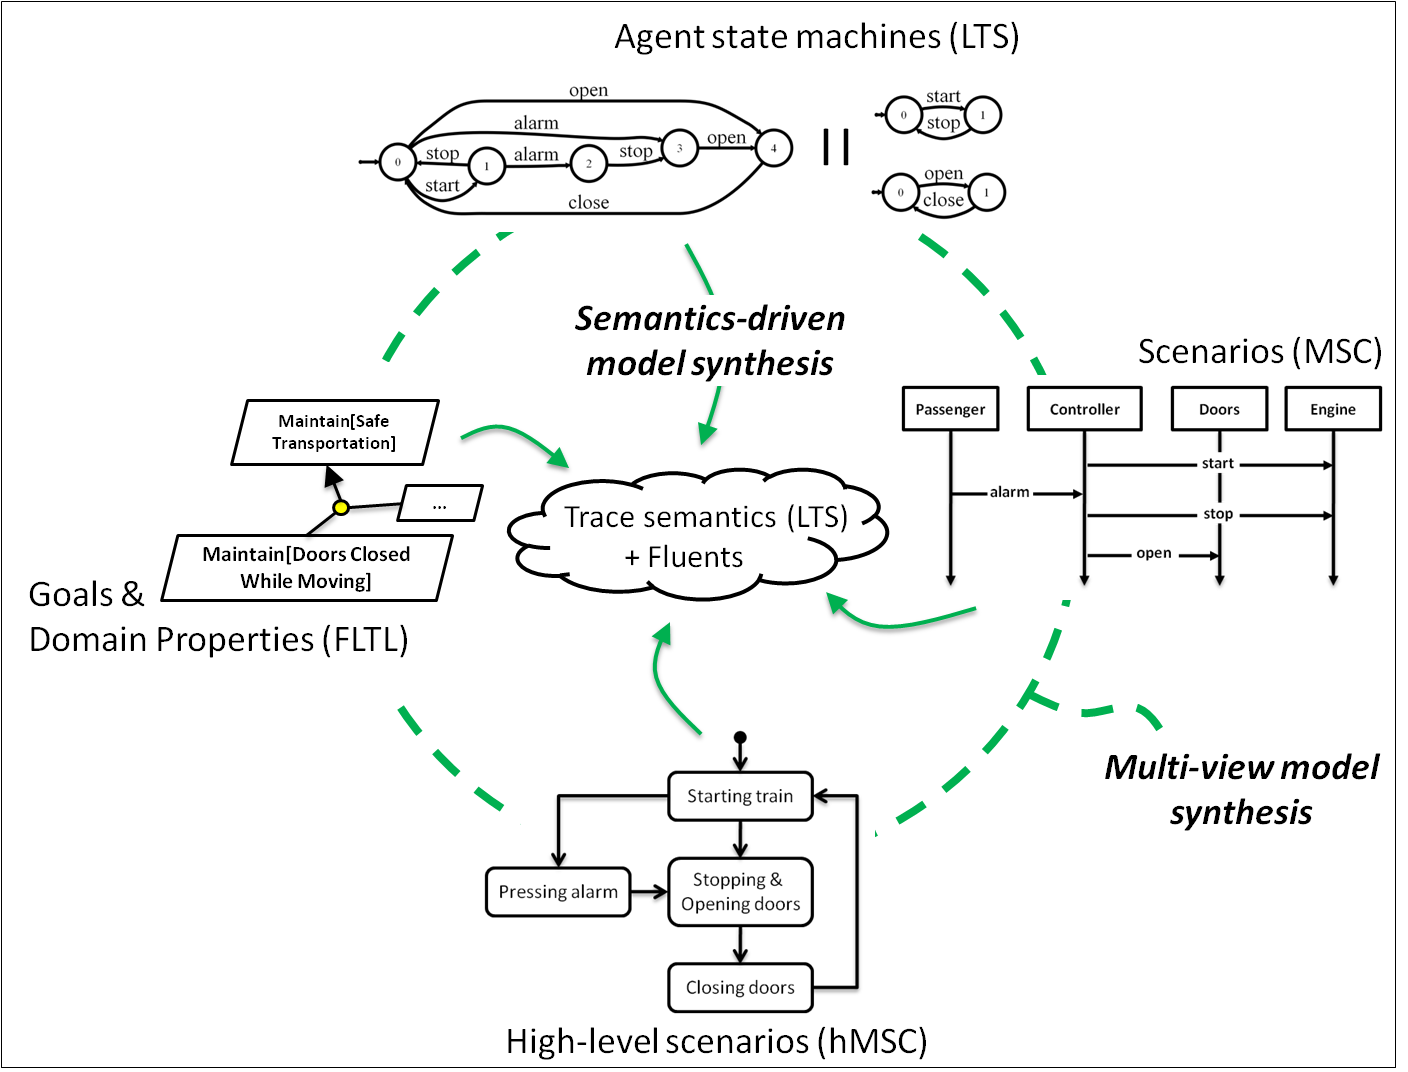
\includegraphics[trim=2mm 2mm 3mm 2mm, clip]{src/2-framework/images/framework}}
  \caption{Formal framework outline.\label{image:framework}}
\end{figure}

The multi-view framework is depicted in Fig.~\ref{image:framework}, that provides a key for reading the rest of this chapter. As we put more emphasis on behavior modeling, all models will be grounded on standard trace theory~\cite{Hoare:1985}. \emph{Traces} are finite sequences of event labels. They will be used to capture the system behaviors described in a MSC scenario, those admitted by a behavioral goal, and so on. Labeled transition systems (LTS) will allow us to capture and manipulate \emph{sets} of traces. A trace-based semantics will provide precise answers to questions such as:
\begin{itemize} 
\item What agent and system traces does this scenario cover?
\item Is this trace accepted by this state machine?
\item Does this sequence of events violate this behavioral goal?
\end{itemize}

Note that labeled transition systems appear twice in the figure as we will make two different uses of them:
\begin{itemize} 
\item LTS provide a representation for the sets of traces that capture model semantics. 
\item They are also chosen as a particular representation for agent state machines\footnote{Even though one could argue that such representation is too low-level to be accessible to stakeholders}.
\end{itemize}

This double use of LTS also illustrates the two different perspectives of behavior model synthesis considered in the thesis:
\begin{itemize}
\item In Chapter~\ref{chapter:deductive}, LTS synthesis is used to capture the semantics of process models and make analyzable;
\item In Chapter~\ref{chapter:inductive-synthesis}, LTS synthesis is used to infer the state machines of system agents from scenarios illustrating interactions among them.
\end{itemize}

